\documentclass[10pt,a4paper]{report}
\usepackage[utf8]{inputenc}
\usepackage[russian]{babel}
\usepackage[OT1]{fontenc}
\usepackage{amsmath}
\usepackage{amsfonts}
\usepackage{amssymb}
\usepackage{graphicx}
\author{Киселев Антон и Кенть Никита}
\title{Отчет по лабораторной работе по дисциплине: "Сети и системы передачи данных"\newline
тема: "Визуализация сигналов во временной и частотной области"}
\date{13.03.14}
\begin{document}
\maketitle
\pagebreak
\chapter{Теоретическая часть}
\section{Цель работы}
Познакомиться со средствами генерации сигналов и визуализации их спектров.
\section{Постановка задачи}
В командном окне MATLAB и в среде Simulink промоделировать чистый синусоидальный сигнал, 
так же синусоидальный сигнал с шумом. Получить их спектры.

\chapter{Ход работы}
\section{Алгоритм работы. Построение сигналов}
\begin{itemize}
\item Построение синусоидального сигнала без шумов
\item Вывод временной характеристики сигнала
\item Реализация  преобразования Фурье 
\item Построение графика спектральной плотности 
\item Построение зашумленного синусоидального сигнала  
\item Вывод временной характеристики полученного сигнала
\item Преобразования Фурье 
\item Построение графика спектральной плотности для зашумленного сигнала
\end{itemize}
\section{Код MATLAB}
function main()\newline
x=0:0.01:4*pi;\newline
t0 = 5;\newline
\%исходный сигнал\newline
y = sin(2*pi*f0*x);\newline
figure(1)\newline
plot(x(1:200),y(1:200))\newline
grid\newline
\%спектр исходного сигнала\newline
figure(2)\newline
spectrum = fft(y,1024);\newline
normspectrum = spectrum.*conj(spectrum)/1024;\newline
f=100*(0:1023)/1024;\newline
plot(f, normspectrum(1:1024))\newline
axis([0 max(f) 0 10])\newline
grid\newline
\%зашумленный сигнал\newline
ynoize = y+ 0.5*rand(size(x));\newline
figure(3)\newline
plot(x(1:200),ynoize(1:200));\newline
grid\newline
\%спектр зашумленного сигнала\newline
spectrum = fft(ynoize,1024);\newline
noizespectrum = spectrum.*conj(spectrum)/1024;\newline
figure(4)\newline
plot(f, noizespectrum())\newline
axis([0 max(f) 0 10])\newline
grid\newline
\section{Результаты работы}
В результате выполнения программы получились графики временной и частотной характеристик исходного и зашумленного синусоидальных сигналов. \newpage
\begin{figure}
\begin{center}
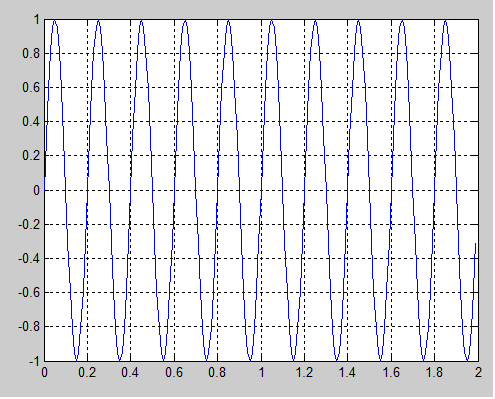
\includegraphics[angle=0, scale = 0.9]{1.png}\newline
рис. 1 Исходный сигнал\newline
\end{center}
\begin{center}
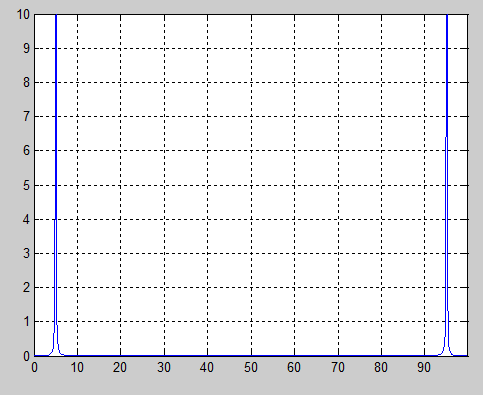
\includegraphics[angle=0, scale = 0.9]{2.png}\newline
рис. 2. Спектр исходного сигнала\newline
\end{center}
\end{figure}
\begin{figure}
\begin{center}
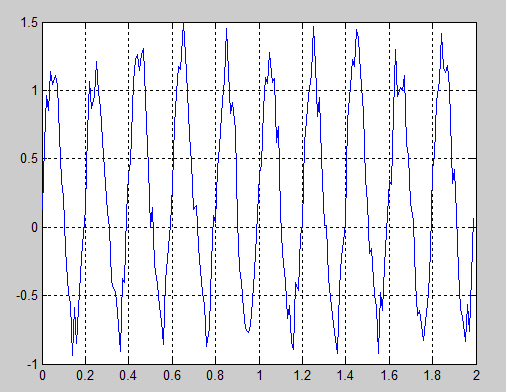
\includegraphics[angle=0, scale = 0.9]{3.png}\newline
рис. 3. Зашумленный сигнал\newline
\end{center}
\begin{center}
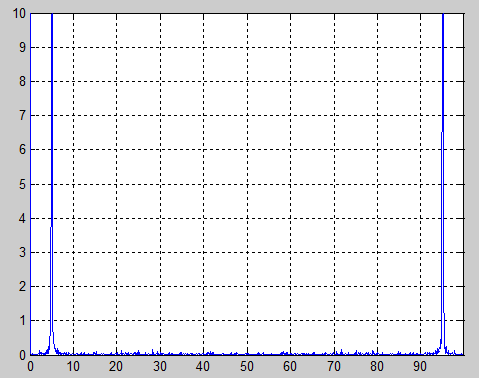
\includegraphics[angle=0, scale = 0.9]{4.png}\newline
рис. 4. Спектр зашумленного сигнала\newline
\end{center}
\end{figure}

\chapter{Построение спектров}
\section{Алгоритм работы}
\begin{itemize}
\item Построение полигармонического сигнала
\item Построение прямоугольного импульсного сигнала
\item Построение треугольного импульсного сигнала
\item Получение спектров этих сигналов
\item Создание моделей в Simulink
\end{itemize}
\section{Код MATLAB}
function laba5()\newline
x = 0:0.01:4*pi;\newline
f0 = 5;\newline
y = 0;\newline
for i=1:1:100\newline
    y=y+cos(i*x);\newline
end\newline
plot(x(1:100),y(1:100));\newline
figure(1)\newline
spectrum=fft(y,512);\newline
normspectrum=spectrum.*conj(spectrum)/512;\newline
f=100*(0:255)/512;\newline
figure(2)\newline
plot(f,normspectrum(1:256))\newline
axis([0 max(f) 0 10])\newline
grid \newline
figure(3)\newline
y1=square(x,50)\newline
plot(x(1:1000),y1(1:1000),'LineWidth',2);\newline
ylim([-1.2,1.2]);\newline
spectrum=fft(y1,512);\newline
normspectrum=spectrum.*conj(spectrum)/512;\newline
f1=100*(0:255)/512;\newline
figure(4)\newline
plot(f1,normspectrum(1:256))\newline
axis([0 max(f1) 0 10])\newline
grid \newline
y2=conv(y1,y1);\newline
figure(5)\newline
plot(x(1:1000),y2(1:1000),'LineWidth',2);\newline
grid\newline
spectrum=fft(y2,512);\newline
normspectrum=spectrum.*conj(spectrum)/512;\newline
f2=100*(0:255)/512;\newline
figure(6)\newline
plot(f2,normspectrum(1:256)/1000)\newline
axis([0 max(f2) 0 10])\newline
grid \newline
end\newline
\section{Результаты работы}
\begin{figure}
\begin{center}
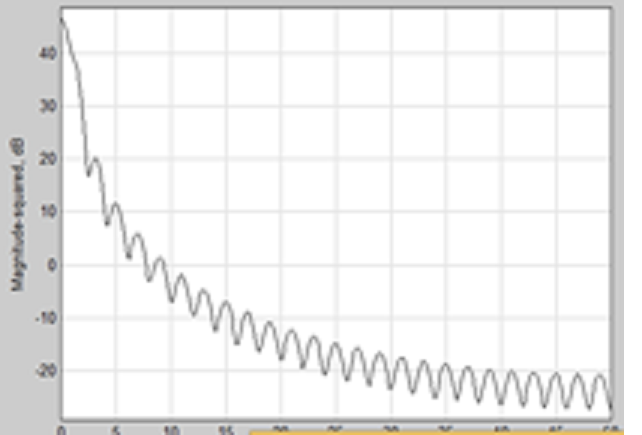
\includegraphics[angle=0, scale = 0.9]{5.png}\newline
рис. 5. спектр прямоугольного сигнала\newline
\end{center}
\end{figure}
\begin{figure}
\begin{center}
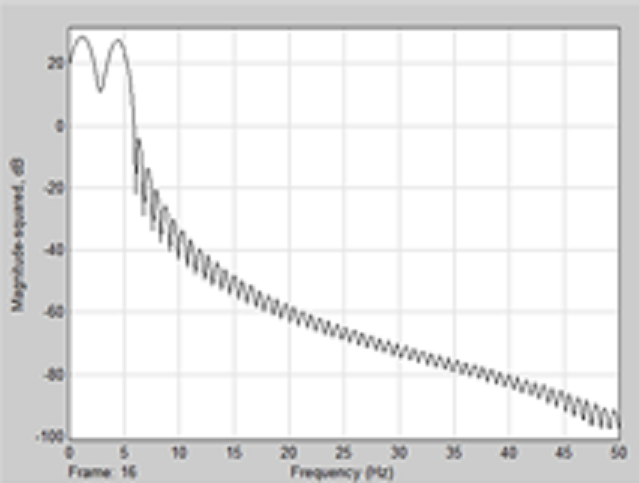
\includegraphics[angle=0, scale = 0.7]{6.png}\newline
рис. 6.спектр полигармонического сигнала\newline
\end{center}
\end{figure}
\begin{figure}
\begin{center}
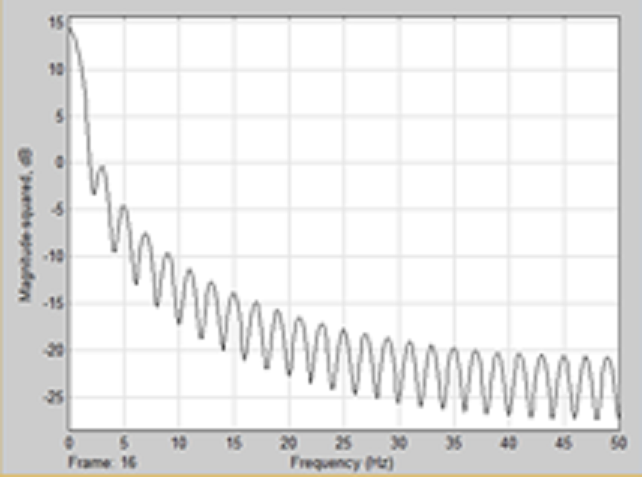
\includegraphics[angle=0, scale = 0.7]{7.png}\newline
рис. 7.спектр треугольного сигнала\newline
\end{center}
\end{figure}
\begin{figure}
\begin{center}
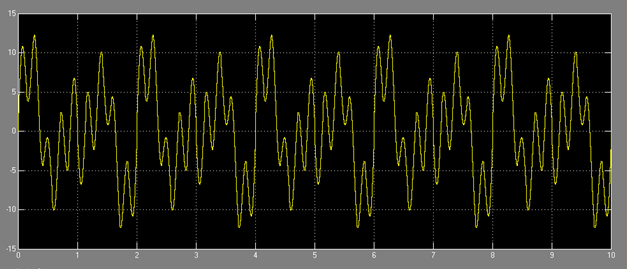
\includegraphics[angle=0, scale = 0.7]{8.png}\newline
рис. 8 полигармонический сигнал\newline
\end{center}
\end{figure}
\begin{figure}
\begin{center}
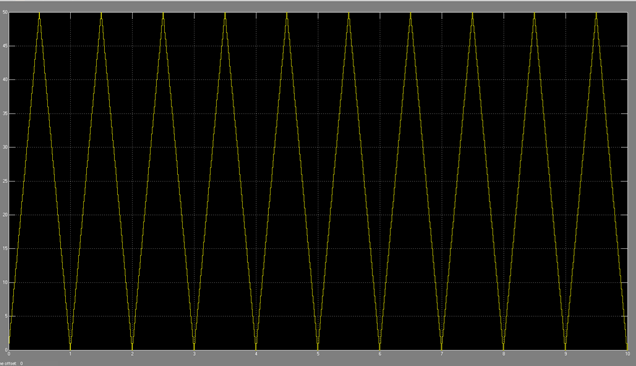
\includegraphics[angle=0, scale = 0.7]{9.png}\newline
рис. 9  треугольный сигнал\newline
\end{center}
\end{figure}
\begin{figure}
\begin{center}
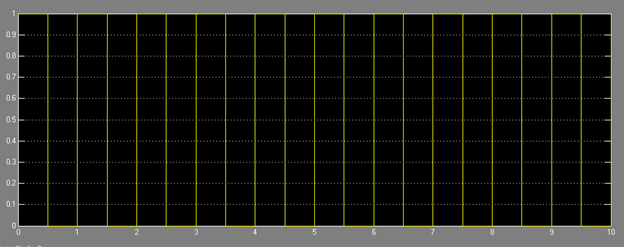
\includegraphics[angle=0, scale = 0.7]{10.png}\newline
рис. 10  прямоугольный сигнал\newline
\end{center}
\end{figure}


\begin{figure}
\begin{center}
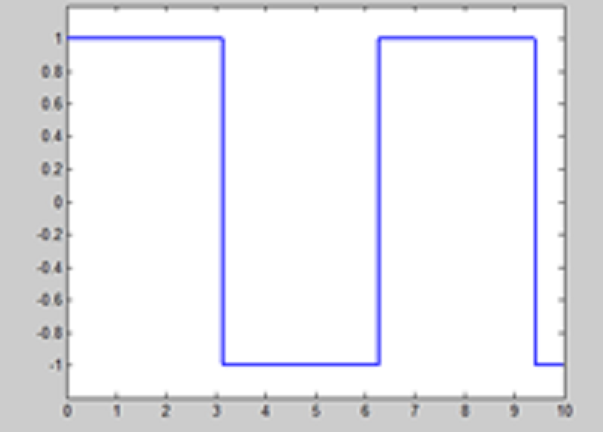
\includegraphics[angle=0, scale = 0.7]{11.png}\newline
рис. 11  прямоугольный сигнал\newline
\end{center}
\end{figure}

\begin{figure}
\begin{center}
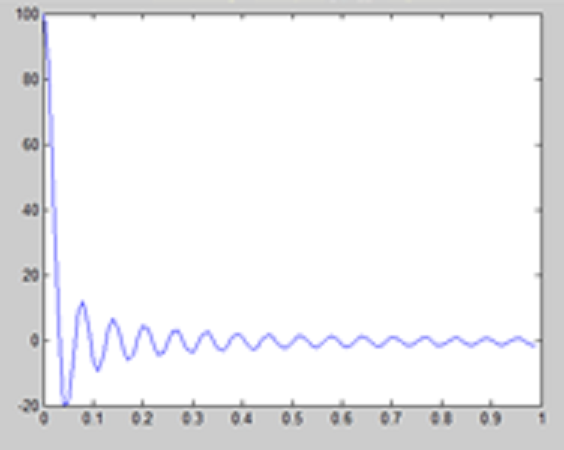
\includegraphics[angle=0, scale = 0.9]{12.png}\newline
рис. 12  полигармонический сигнал\newline
\end{center}
\end{figure}
\begin{figure}
\begin{center}
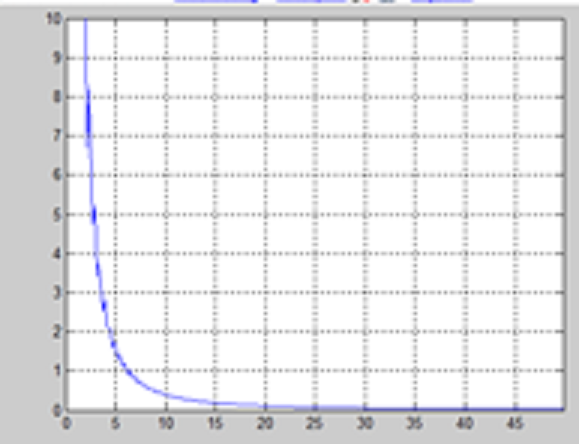
\includegraphics[angle=0, scale = 0.9]{13.png}\newline
рис. 13   спектр треугольного сигнала\newline
\end{center}
\end{figure}

\begin{figure}
\begin{center}
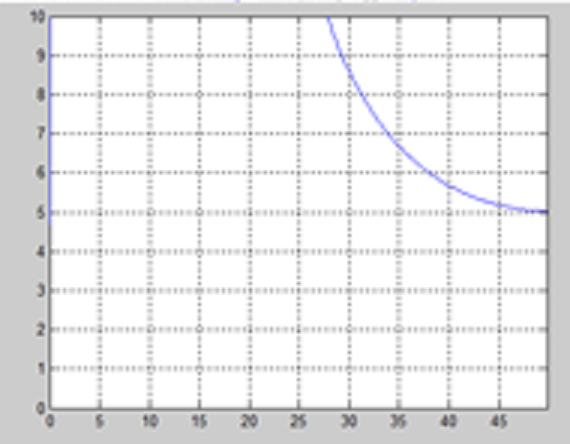
\includegraphics[angle=0, scale = 0.9]{14.png}\newline
рис. 14   спектр прямоугольного сигнала\newline
\end{center}
\end{figure}

\begin{figure}
\begin{center}
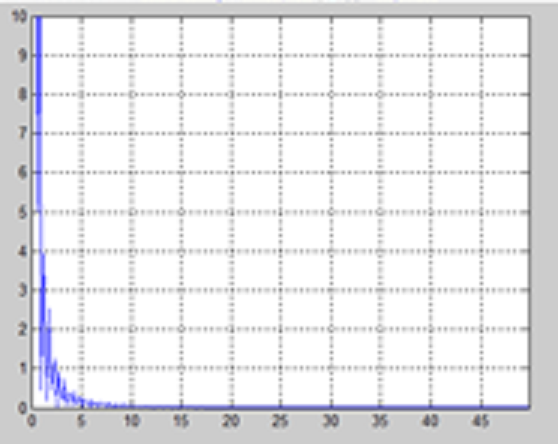
\includegraphics[angle=0, scale = 0.79]{15.png}\newline
рис. 15    спектр полигармонического сигнала\newline
\end{center}
\end{figure}

\begin{figure}
\begin{center}
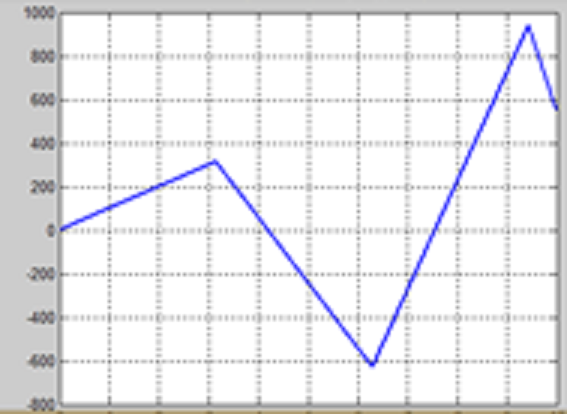
\includegraphics[angle=0, scale = 0.9]{16.png}\newline
рис. 16    треугольный сигнал\newline
\end{center}
\end{figure}
\chapter{Вывод}
В данной лабораторной работе были проведедены исследования по получению спектров исходного сигнала и сигнала с шумом. Исходный сигнал вычислялся на конечном промежутке и дискретном наборе с определенной частотой квантования. По полученнным практическим результатам спектр исходного сигнала получился периодическим, что соответствует ожидаемым теоретическим результатам. Спектр получается периодическим по частоте, так как в результате разложения сигнала в ряд Фурье он умножается на комплексную экспоненту, которая обладает свойством периодичности.Спектр конечного дискретного сигнала определяется своей равномерной дискретной выборкой с постоянной частотой дискретизации Dw, то есть спектр определяется конечным числом гармоник на частотах k*DW.. \newline

В следующей лабораторной работе было проведено моделирование полигармонического сигнала

 прямоугольного сигнала и треугольного сигнала. Были получены спектры данных сигналов. Для получения сигналов использовались математические формулы данных функций, а также средство моделирования Simulink. Обоими способами были получены спектры сигналов. Частным случаем в работе было получение треугольного сигнала через премение операции свертки над произведением двух прямоуголных сигналов. Данная операция осуществляется как математически, так и при моделировании в среде Simulink.
Обоснованием получения треугольного сигнала из свертки двух прямоугольных служит тот факт, что интеграл от произведения двух констант есть линейная функция. График такого преобразования будет представлять две линеных функции, одна из котрых имеет положительный коэффициента наклона, а другая отрицательный.
\begin{figure}
\begin{center}
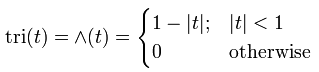
\includegraphics[angle=0, scale = 0.8]{17.png}\newline
рис. 17    Формула полигармонического сигнала\newline
\end{center}
\end{figure}
\begin{figure}
\begin{center}
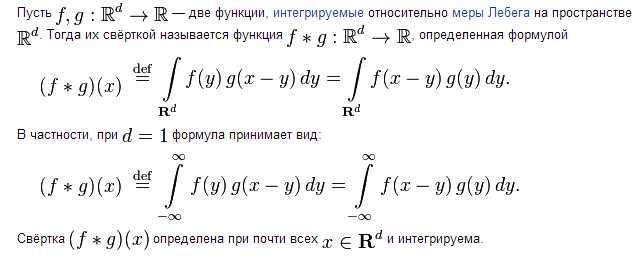
\includegraphics[angle=0, scale = 0.8]{18.png}\newline
рис. 18   Свертка функций
\end{center}
\end{figure}
\begin{figure}
\begin{center}
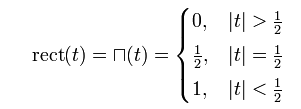
\includegraphics[angle=0, scale = 0.8]{19.png}\newline
рис. 19    Прямоугольная функция
\end{center}
\end{figure}
\begin{figure}
\begin{center}
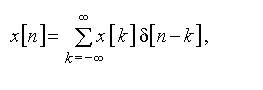
\includegraphics[angle=0, scale = 0.8]{20.png}\newline
рис. 20   Дискретный сигнал
\end{center}
\end{figure}
\begin{figure}
\begin{center}
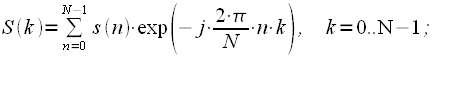
\includegraphics[angle=0, scale = 0.8]{21.png}\newline
рис. 21    Спектр дискретного сигнала
\end{center}
\end{figure}
\end{document}
